\documentclass[12pt, a4paper]{article}

\usepackage[margin=1.15in]{geometry}
\usepackage{xcolor}
\usepackage{mdframed}
\usepackage{titlesec}
\usepackage{fancyhdr}
\usepackage{enumitem}
\usepackage{booktabs}
\usepackage{array}
\usepackage{microtype}
\usepackage{hyperref}
\usepackage{tikz}
\usetikzlibrary{arrows.meta, positioning, shapes.geometric, backgrounds, calc}
\usepackage{graphicx}
\usepackage{setspace}
\usepackage{fontenc}

% --- Colors ---
\definecolor{pigreen}{RGB}{0, 130, 60}
\definecolor{piamber}{RGB}{190, 110, 0}
\definecolor{piblue}{RGB}{30, 80, 160}
\definecolor{pigray}{RGB}{90, 90, 90}
\definecolor{pilight}{RGB}{242, 250, 245}
\definecolor{piyellow}{RGB}{255, 250, 225}
\definecolor{piborder}{RGB}{0, 100, 50}
\definecolor{amberborder}{RGB}{180, 100, 0}
\definecolor{blueborder}{RGB}{20, 60, 140}
\definecolor{redborder}{RGB}{160, 30, 30}
\definecolor{pired}{RGB}{200, 40, 40}

% --- Hyperref ---
\hypersetup{colorlinks=true, linkcolor=pigreen, urlcolor=pigreen}

% --- Header/Footer ---
\pagestyle{fancy}
\fancyhf{}
\rhead{\textcolor{pigray}{\small\textit{Pi$^2$ Cipher — Plain English Guide}}}
\lhead{\textcolor{pigray}{\small\textit{DRAFT}}}
\cfoot{\textcolor{pigray}{\thepage}}
\renewcommand{\headrulewidth}{0.4pt}

% --- Section styling ---
\titleformat{\section}{\large\bfseries\color{pigreen}}{}{0em}{}[\vspace{-0.2em}\textcolor{piborder}{\rule{\linewidth}{0.5pt}}]
\titleformat{\subsection}{\normalsize\bfseries\color{pigray}}{}{0em}{}

% --- Callout boxes ---
\newmdenv[linecolor=piborder, backgroundcolor=pilight, linewidth=1.2pt,
  innerleftmargin=14pt, innerrightmargin=14pt, innertopmargin=10pt,
  innerbottommargin=10pt, roundcorner=4pt]{greenbox}

\newmdenv[linecolor=amberborder, backgroundcolor=piyellow, linewidth=1.2pt,
  innerleftmargin=14pt, innerrightmargin=14pt, innertopmargin=10pt,
  innerbottommargin=10pt, roundcorner=4pt]{amberbox}

\newmdenv[linecolor=blueborder, backgroundcolor={rgb:blue,1;white,8}, linewidth=1.2pt,
  innerleftmargin=14pt, innerrightmargin=14pt, innertopmargin=10pt,
  innerbottommargin=10pt, roundcorner=4pt]{bluebox}

\newmdenv[linecolor=redborder, backgroundcolor={rgb:red,1;white,10}, linewidth=1.2pt,
  innerleftmargin=14pt, innerrightmargin=14pt, innertopmargin=10pt,
  innerbottommargin=10pt, roundcorner=4pt]{redbox}

% ============================================================
\begin{document}
% ============================================================

% --- Title Page ---
\begin{titlepage}
\centering
\vspace*{1.8cm}

{\fontsize{52}{60}\selectfont $\pi^2$}\\[0.5em]
{\Huge\bfseries\color{pigreen} Cipher}\\[0.7em]
{\large\color{pigray} A New Encryption System Built on the Digits of Pi}

\vspace{1.2cm}
\textcolor{piborder}{\rule{0.55\linewidth}{1pt}}
\vspace{1.2cm}

{\large\textbf{Proof of Concept}}\\[0.4em]
{\large\textit{Plain English Edition}}\\[0.8em]
{\color{pigray} Version 0.1 — \today}

\vspace{1.8cm}

\begin{amberbox}
\centering\small\color{piamber}
\textbf{WHO THIS IS FOR}\\[0.4em]
\color{pigray}
This document explains the Pi$^2$ Cipher to anyone curious about how it works ---
no mathematics degree required. Technical terms are explained as they appear.
The goal is simple: by the end, you should be able to explain this cipher
to a friend over coffee.
\end{amberbox}

\vfill
{\small\color{pigray}
This is an experimental research concept. Not intended for production use.
}
\end{titlepage}

\tableofcontents
\newpage

% ============================================================
\section{The Big Idea in One Paragraph}
% ============================================================

\vspace{0.5em}

The number pi ($\pi$ = 3.14159265358979...) goes on forever with no pattern and no repetition. Every digit, 0 through 9, appears roughly the same number of times. Mathematicians believe --- and have checked for over ten trillion digits --- that pi looks completely random, even though it is a fixed, defined number. The Pi$^2$ Cipher uses this infinite, random-looking sequence as the source of all its scrambling power. Your secret key tells the cipher \textit{where} to look inside pi. Without the key, an attacker has no idea where to look --- and since pi is infinite, there is nowhere to even begin guessing.

\begin{greenbox}
\textbf{One-line summary:} Your key is a secret address inside an infinite, random-looking book. The cipher opens the book at that address, collects the scrambling ingredients, and uses them to lock your message.
\end{greenbox}

% ============================================================
\section{The Problem This Solves}
% ============================================================

\vspace{0.5em}

Every day, billions of messages are encrypted --- bank transfers, text messages, passwords, medical records. Encryption works by scrambling a message so thoroughly that only someone with the right key can unscramble it.

The current gold standard for encryption is called AES (Advanced Encryption Standard). It was designed in the late 1990s, adopted by the US government in 2001, and has been used worldwide ever since. AES is trusted and well-studied, but it has one notable property: \textbf{all of its internal scrambling rules are public}. Anyone in the world can look up exactly how AES scrambles data. The only secret is the key.

This is actually a deliberate design choice --- it means the security depends entirely on the key, not on keeping the scrambling method secret. But it also means that anyone trying to break AES already knows the rulebook. They just need to find the key.

\begin{bluebox}
\textbf{What if the rulebook was secret too?} That is the central question behind the Pi$^2$ Cipher. Here, the scrambling rules themselves are derived from your secret key via the digits of pi. An attacker does not know the key \textit{and} does not know the rules that were used. They are trying to solve a puzzle without even knowing what kind of puzzle it is.
\end{bluebox}

% ============================================================
\section{Pi: The World's Best Random Number Generator}
% ============================================================

\vspace{0.5em}

Before explaining the cipher, it helps to understand why pi is special here.

\subsection{Pi never ends and never repeats}

Unlike $\frac{1}{3}$ = 0.333... which repeats, or $\frac{1}{4}$ = 0.25 which ends, pi goes on forever with no repeating block. The digits look statistically random --- any string of numbers you can think of (your phone number, your birthday, any sequence) appears somewhere in pi, and will appear again infinitely many times.

\subsection{You can jump to any digit directly}

Here is something remarkable: there exists a mathematical formula (called the BBP formula, discovered in 1995) that lets you calculate the ten-trillionth digit of pi \textit{without first calculating all the digits before it}. You can jump straight to any position.

\begin{greenbox}
\textbf{Why this matters:} Our cipher needs to look up digits of pi at random, very large positions --- positions like 7,341,829,204,918. The BBP formula makes this practical. We do not need to store trillions of digits; we can compute any one digit on demand.
\end{greenbox}

\subsection{Pi is conjectured to be ``normal''}

A ``normal'' number is one where every digit appears equally often, every pair of digits appears equally often, every triple, and so on --- at every scale, the distribution is perfectly uniform. Mathematicians strongly believe pi is normal, and over ten trillion digits have been checked with results consistent with normality. But --- and this is important --- \textbf{it has never been proven}. This is the one unproven assumption the Pi$^2$ Cipher relies on.

% ============================================================
\section{The Key: A Secret Address in Pi}
% ============================================================

\vspace{0.5em}

Your secret key in the Pi$^2$ Cipher is a 256-bit number --- that is a number with 77 digits. This is astronomically large: there are more possible keys than there are atoms in the observable universe.

But the key is not used directly to scramble your message. Instead, it goes through two stages.

\subsection{Stage 1: Hiding the Starting Point}

First, the key is processed by a function called SHA-256. Think of SHA-256 as a blender: you put your key in, and out comes a completely scrambled version of it. Even changing one digit of the key produces a totally different output. This scrambled version becomes your \textbf{starting address} in pi.

\begin{amberbox}
\textbf{Why this step?} If we used the key directly as an address in pi, an attacker could try addresses one by one in order. SHA-256 makes the starting address completely unpredictable from the key, closing that door.
\end{amberbox}

\subsection{Stage 2: Layer 1 --- Finding the Real Addresses}

Starting at the SHA-256 output position, we read pi's digits and group them into chunks of 15. Each chunk of 15 digits forms a new, very large address --- a number up to about 1,150,000,000,000,000,000. We generate 46 of these addresses.

Think of it like this: your key gives you one address. That address is a page in the pi book. On that page, you find 46 more addresses written in pi's digits.

\subsection{Stage 3: Layer 2 --- Collecting the Ingredients}

Now we use those 46 addresses to jump to different locations in pi and extract digits from each one. These digits become our actual scrambling ingredients: the secret codebooks, the mixing rules, and the round keys used during encryption.

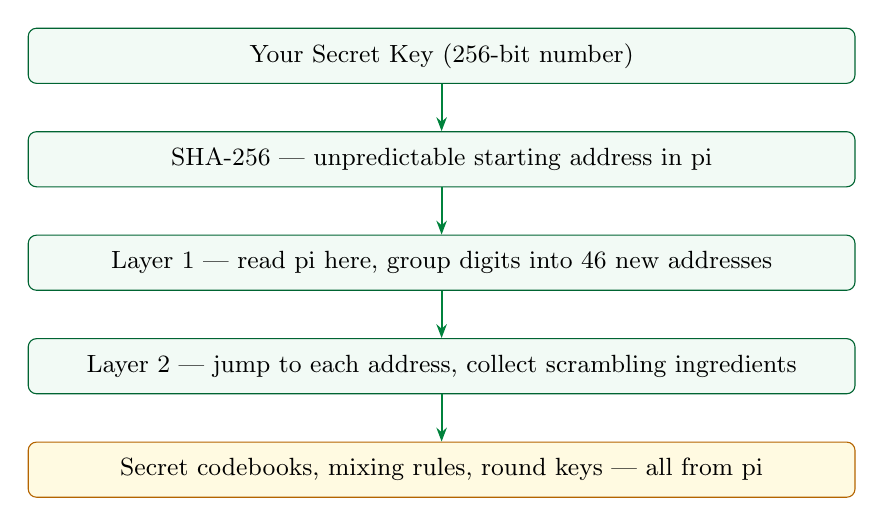
\begin{tikzpicture}[
  node distance=0.6cm,
  box/.style={rectangle, draw=piborder, fill=pilight, rounded corners=3pt,
              minimum width=5cm, minimum height=0.7cm, align=center, font=\small},
  arr/.style={-{Stealth[length=5pt]}, color=pigreen, thick},
  wide/.style={rectangle, draw=piborder, fill=pilight, rounded corners=3pt,
               minimum width=10.5cm, minimum height=0.7cm, align=center, font=\small}
]
\node[wide] (key) {Your Secret Key (256-bit number)};
\node[wide, below=of key] (sha) {SHA-256 --- unpredictable starting address in pi};
\node[wide, below=of sha] (l1) {Layer 1 --- read pi here, group digits into 46 new addresses};
\node[wide, below=of l1] (l2) {Layer 2 --- jump to each address, collect scrambling ingredients};
\node[wide, below=of l2, draw=amberborder, fill=piyellow] (mat) {Secret codebooks, mixing rules, round keys --- all from pi};

\draw[arr] (key) -- (sha);
\draw[arr] (sha) -- (l1);
\draw[arr] (l1) -- (l2);
\draw[arr] (l2) -- (mat);
\end{tikzpicture}

\vspace{0.8em}

This double-jump structure --- using pi to find where to look in pi --- is what gives the cipher its name. Pi squared. Pi pointing to itself.

% ============================================================
\section{Encrypting the Message: 14 Rounds of Scrambling}
% ============================================================

\vspace{0.5em}

Once the ingredients are collected, the actual encryption begins. Your message is broken into blocks --- each block is a grid of 64 numbers arranged in an 8-by-8 square. Each number represents one letter or character. Then the block goes through \textbf{14 rounds} of scrambling.

Think of each round as a machine with five stations inside. Your block of text passes through all five stations, comes out the other end, and immediately enters the next machine. After 14 machines, it is unrecognizable.

\subsection{Station 1: PiSubBytes --- Swap Every Character}

A substitution table is a lookup list: ``whenever you see the number 42, replace it with 187. Whenever you see 7, replace it with 231.'' Every possible input (0 to 255) maps to a unique output.

In standard AES, this table is fixed and public. In the Pi$^2$ Cipher, \textbf{the table is generated fresh for every round from pi digits}. It is different each round, and different for every key. An attacker cannot precompute attacks against it because they do not know what table was used.

\begin{greenbox}
\textbf{Analogy:} Imagine swapping letters using a secret decoder ring. AES uses the same decoder ring that everyone has seen. Pi$^2$ Cipher generates a new decoder ring --- one that only exists for your key, for this message, for this round.
\end{greenbox}

\subsection{Station 2: PiShiftRows --- Rearrange the Grid}

The 8-by-8 grid has 8 rows. Each row gets slid sideways by a certain number of positions. In AES, the slide amounts are always the same: row 1 slides 0 places, row 2 slides 1 place, row 3 slides 2 places, row 4 slides 3 places. Public and fixed.

In the Pi$^2$ Cipher, the slide amounts for all 8 rows are determined by pi digits from your key. An attacker does not know how far each row was shifted.

\subsection{Station 3: MixColumns --- Blend the Columns}

After substitution and shifting, each column of 8 numbers gets mathematically blended together using a mixing matrix --- a grid of numbers that combines the column into a new column where every output depends on every input.

The mixing matrix must satisfy a mathematical property called MDS (Maximum Distance Separable). This is a guarantee that changing even one number in the column will completely change all 8 numbers in the output. This property ensures that changes in your message spread out and affect the entire block, not just one part of it.

In AES, the MDS matrix is fixed and public. In Pi$^2$ Cipher, it is generated from pi and verified to satisfy the MDS property before use.

\subsection{Station 4: PiKeyMix --- Inject Fresh Pi Randomness}

This station does not exist in AES. After the blending step, we XOR the entire block with 32 fresh bytes pulled directly from pi at a round-specific position.

XOR is a simple operation: for each bit, if the two bits are the same the result is 0; if they are different the result is 1. It is its own inverse --- apply it twice with the same number and you get back to where you started. This is how decryption works.

This extra injection of pi-based randomness between every round adds a layer of security that is completely independent of the algebraic structure of the other steps.

\subsection{Station 5: AddRoundKey --- Lock in the Key}

The final station in each round XORs the block with a 32-byte round key extracted from pi via the key schedule. This is the step that ties everything to the secret key. Without the key, you cannot reverse this step.

\begin{bluebox}
\textbf{After 14 rounds:} Every bit of the ciphertext depends on every bit of the plaintext, every bit of the key, and many digits of pi at positions that only your key can locate. Changing one letter in the original message changes approximately half the bits in the output --- this is called the avalanche effect, and it is the hallmark of a strong cipher.
\end{bluebox}

% ============================================================
\section{Decryption: Running it Backwards}
% ============================================================

\vspace{0.5em}

Every station in the cipher is reversible. The receiver, who knows the secret key, can regenerate all the same pi-derived ingredients and run the process in reverse:

\begin{center}
\renewcommand{\arraystretch}{1.4}
\begin{tabular}{ll}
\toprule
\textbf{Encryption Step} & \textbf{How to Reverse It} \\
\midrule
PiSubBytes & Apply the inverse substitution table (swap back) \\
PiShiftRows & Shift each row back by the same amount in the other direction \\
MixColumns & Multiply by the mathematical inverse of the mixing matrix \\
PiKeyMix & XOR with the same pi bytes again (XOR is self-reversing) \\
AddRoundKey & XOR with the same round key again \\
\bottomrule
\end{tabular}
\end{center}

\vspace{0.5em}
The receiver regenerates the same key schedule from the same seed and nonce, runs the same BBP formula to compute the same pi digits, and the decryption is perfect.

% ============================================================
\section{Why Is This Hard to Break?}
% ============================================================

\vspace{0.5em}

Let us think like an attacker. They have the ciphertext. They want the plaintext. What can they try?

\subsection{Guess the key}

The key is a 256-bit number. There are $2^{256}$ possible keys --- roughly $10^{77}$. Even if you could check one trillion keys per second and ran every computer on Earth for the entire age of the universe, you would not get through a measurable fraction of the possibilities.

\subsection{Work backwards from the ciphertext}

To reverse the encryption, you need to know: the substitution tables, the shift amounts, the mixing matrix, and the round keys. But all of these come from pi via the secret key. Without the key, you do not know any of them. And they are all different every time --- different key, different message, different block.

\subsection{Look for patterns}

Strong ciphers are designed so the ciphertext looks like pure random noise. Because the Pi$^2$ Cipher uses a pi-derived MDS matrix and 14 rounds of mixing, every output bit depends on every input bit in a non-linear way. There are no detectable patterns.

\subsection{Attack the structure}

The classical attacks on block ciphers --- differential cryptanalysis and linear cryptanalysis --- work by exploiting known properties of the fixed S-box and mixing matrix. In AES, these are public, so researchers have had decades to analyze them and confirm they hold up. In Pi$^2$ Cipher, the S-box and mixing matrix are secret and change per key. The attacker cannot build attack tables without first recovering the key --- which is circular.

\begin{redbox}
\textbf{The one weakness to be honest about:} The security of Pi$^2$ Cipher depends on pi being normal --- that its digits are truly random-looking. This is strongly believed and computationally verified for trillions of digits, but it has never been mathematically proven. If someone proved pi is \textit{not} normal, or found a structural pattern in its digits, this cipher could be weakened. This is the acknowledged open assumption in the design.
\end{redbox}

% ============================================================
\section{How Pi\textsuperscript{2} Cipher Compares to AES}
% ============================================================

\vspace{0.5em}

\begin{center}
\renewcommand{\arraystretch}{1.5}
\begin{tabular}{p{5cm}p{3.8cm}p{3.8cm}}
\toprule
\textbf{Feature} & \textbf{AES} & \textbf{Pi$^2$ Cipher} \\
\midrule
Block size & 128 bits & 256 bits \\
Number of rounds & 10 to 14 & 14 \\
Substitution table & Fixed, public & Secret, changes per round \\
Row shift amounts & Fixed, public & Secret, key-derived \\
Mixing matrix & Fixed, public & Secret, key-derived \\
Extra mixing step & None & PiKeyMix every round \\
Years of public analysis & 25+ years & Not yet analyzed \\
Security assumption & Mathematical structure & Pi normality + SHA-256 \\
Relies on single constant & No & Yes (pi) \\
\bottomrule
\end{tabular}
\end{center}

\vspace{0.5em}

The tradeoff is straightforward: Pi$^2$ Cipher has more secret moving parts than AES, which is theoretically an advantage. But AES has been subjected to decades of intense public scrutiny by the world's best cryptographers. Pi$^2$ Cipher has not. In practice, a well-analyzed cipher with public internals is often more trustworthy than a newer, more complex one --- because unknown ciphers can have unknown weaknesses.

% ============================================================
\section{The Nonce: Making Sure Every Message is Unique}
% ============================================================

\vspace{0.5em}

A critical rule in any cipher: \textbf{never encrypt two different messages with the exact same key material}. If you did, an attacker could XOR the two ciphertexts together and the key material would cancel out, leaving a direct relationship between the two plaintexts --- a major leak.

The Pi$^2$ Cipher solves this with a \textbf{nonce} --- a number used once. The nonce is a random public value attached to each message. It gets mixed into the key schedule alongside the secret seed:

\vspace{0.3em}
\begin{center}
\textit{Effective Key Material} = SHA-256(secret seed + nonce + block number)
\end{center}
\vspace{0.3em}

Even with the same secret seed, every message gets a unique nonce, which produces completely different pi lookup positions, which produces completely different scrambling ingredients. The nonce is not secret --- it travels with the ciphertext --- but without the secret seed it is useless to an attacker.

% ============================================================
\section{A Full Example, Step by Step}
% ============================================================

\vspace{0.5em}

Let us walk through encrypting the word ``HELLO'' at a very high level.

\begin{enumerate}[leftmargin=*, label=\textbf{Step \arabic*.}]

  \item \textbf{Pad the message.} ``HELLO'' is 5 characters. We need a full 64-character block (8$\times$8), so we pad it to 64 characters with standard padding. The block is arranged as an 8$\times$8 grid of numbers.

  \item \textbf{Generate the effective seed.} We run SHA-256 on (your secret key + a random nonce). The output is our starting address in pi.

  \item \textbf{Layer 1.} We read pi starting at that address and group digits into 46 large position numbers.

  \item \textbf{Layer 2.} We use those 46 positions to jump around pi and collect 14 round keys, 14 substitution tables, 14 sets of shift amounts, and 1 mixing matrix.

  \item \textbf{Initial key lock.} We XOR the block with round key zero. This immediately ties the block to the secret key.

  \item \textbf{Rounds 1 to 13.} Each round: substitute every number using the secret table, shift the rows, blend the columns with the MDS matrix, inject fresh pi bytes, XOR with the round key.

  \item \textbf{Final round 14.} Substitute, shift rows, XOR with the final round key. No blending step in the final round.

  \item \textbf{Output.} The result is 64 bytes of ciphertext. ``HELLO'' has become something like: \texttt{a7 3f 91 b2 04 e8 5c 19 ...} --- noise with no trace of the original.

  \item \textbf{Send.} The recipient receives the ciphertext and the public nonce. Using the same secret seed, they regenerate all the same pi-derived ingredients and reverse each step. Out comes ``HELLO''.

\end{enumerate}

% ============================================================
\section{What Needs to Happen Next}
% ============================================================

\vspace{0.5em}

This document is a proof of concept --- a demonstration that the idea is coherent and the design is sound. Before this cipher could be used for anything real, several things would need to happen:

\begin{enumerate}[leftmargin=*, label=\arabic*., itemsep=4pt]
  \item \textbf{Formal security proof.} A mathematical proof that the cipher is secure under the stated assumptions, in a standard security model used by cryptographers.

  \item \textbf{Public cryptanalysis.} Publication and review by the cryptography research community. Good ciphers survive years of attempts to break them.

  \item \textbf{Efficient implementation.} The BBP formula for computing pi digits is slower than a simple table lookup. A production implementation would need careful optimization, and possibly hardware acceleration for large pi indices.

  \item \textbf{Progress on pi normality.} Any mathematical advance on proving (or disproving) pi's normality would directly affect the cipher's security foundations.

  \item \textbf{Side-channel analysis.} Modern cipher implementations also need to resist timing attacks, power analysis, and cache-based attacks. This has not been studied for Pi$^2$ Cipher.
\end{enumerate}

% ============================================================
\section{Summary}
% ============================================================

\vspace{0.5em}

\begin{greenbox}
\textbf{The Pi$^2$ Cipher in six sentences:}

\vspace{0.5em}
Pi is an infinite sequence of digits that looks completely random. The Pi$^2$ Cipher uses your secret key to locate specific positions in pi and extract scrambling ingredients from those positions. Those ingredients --- substitution tables, shift amounts, a mixing matrix, and round keys --- are all secret and unique to your key. Your message is then scrambled through 14 rounds of substitution, shifting, blending, and key-locking, producing ciphertext that looks like pure noise. Only someone with the same secret key can regenerate the same pi-derived ingredients and reverse the process. The cipher is as hard to break as the number pi is unpredictable --- which, after ten trillion verified digits, appears to be very hard indeed.
\end{greenbox}

\vspace{1.5em}

\begin{amberbox}
\textbf{The one open question everything rests on:}\\[0.4em]
\color{pigray}
Is pi truly normal? Are its digits genuinely, provably random at every scale? Mathematicians believe the answer is yes. Nobody has proven it. Until they do, the Pi$^2$ Cipher rests on the same mystery that has fascinated mathematicians for centuries --- the true nature of the most famous number in the world.
\end{amberbox}

% ============================================================
\newpage
\section*{Glossary}
% ============================================================
\addcontentsline{toc}{section}{Glossary}

\renewcommand{\arraystretch}{1.6}
\begin{tabular}{p{3.5cm}p{9.5cm}}
\toprule
\textbf{Term} & \textbf{Plain English meaning} \\
\midrule
AES & The current world standard for encryption, used in banking, messaging, and government systems. \\
BBP Formula & A mathematical trick that computes any specific digit of pi directly, without computing all digits before it. \\
Block cipher & An encryption system that works on fixed-size chunks of data at a time. \\
Ciphertext & The scrambled, unreadable output of encryption. \\
Diffusion & The property that changing one part of the input changes many parts of the output. \\
GF(2$^8$) & A mathematical number system with exactly 256 elements, used for the mixing step. \\
MDS matrix & A mixing table with a proven guarantee that any change to the input spreads to every output. \\
Nonce & A random number used once, attached to each message to ensure unique key material. \\
Normal number & A number whose digits are statistically uniform at every scale --- like a perfect random source. \\
Pi ($\pi$) & The ratio of a circle's circumference to its diameter: 3.14159265... continuing forever. \\
Plaintext & The original, readable message before encryption. \\
PRF & Pseudorandom Function --- a function that produces outputs indistinguishable from random noise. \\
Round & One complete pass through all five scrambling stations. Pi$^2$ uses 14 rounds. \\
SHA-256 & A standard mathematical blender: any input produces a fixed, unpredictable output. \\
S-box & Substitution box --- a lookup table that swaps one number for another during encryption. \\
XOR & A simple bit operation that is its own inverse: apply it twice and you undo it. \\
\bottomrule
\end{tabular}

\end{document}
